\documentclass[11pt]{article}

\usepackage[T1]{fontenc}
\usepackage[utf8]{inputenc}
\usepackage{lmodern}
\usepackage{microtype}
\usepackage[left=0.85in,right=1.35in,top=0.78in,bottom=0.82in,headheight=15pt]{geometry}
\usepackage{amsmath,amssymb}
\usepackage{booktabs,longtable,tabularx,array}
\usepackage[dvipsnames]{xcolor}
\usepackage{enumitem}
\usepackage{fancyhdr}
\usepackage{hyperref}
\usepackage{tikz}
\usetikzlibrary{arrows.meta,positioning}

\definecolor{navy}{HTML}{17365D}
\definecolor{teal}{HTML}{137C8B}
\definecolor{green}{HTML}{176B3A}
\definecolor{greenbg}{HTML}{E7F4EC}
\definecolor{amber}{HTML}{8A5A00}
\definecolor{amberbg}{HTML}{FFF4D6}
\definecolor{red}{HTML}{9A2D2D}
\definecolor{redbg}{HTML}{FBE9E7}
\definecolor{graybg}{HTML}{F3F5F7}
\definecolor{linegray}{HTML}{D7DDE3}

\hypersetup{
  colorlinks=true,
  linkcolor=navy,
  urlcolor=teal,
  pdftitle={Mortensen-Pissarides (1994): Theorem and Proof Progress Audit},
  pdfauthor={Lean4Tutorial audit}
}

\pagestyle{fancy}
\fancyhf{}
\fancyhead[L]{\small MP1994 theorem progress}
\fancyhead[R]{\small Human review audit}
\fancyfoot[C]{\thepage}

\setlength{\parindent}{0pt}
\setlength{\parskip}{0.48em}
\setlength{\LTpre}{0.35em}
\setlength{\LTpost}{0.7em}
\setlist{nosep,leftmargin=1.4em}
\renewcommand{\arraystretch}{1.15}
\sloppy

\newcommand{\code}[1]{\nolinkurl{#1}}
\newcommand{\src}[1]{\nolinkurl{#1}}
\newcommand{\chip}[2]{\colorbox{#1}{\strut\scriptsize\textbf{#2}}}
\newcommand{\pf}{\chip{greenbg}{PF}}
\newcommand{\pc}{\chip{amberbg}{PC}}
\newcommand{\en}{\chip{amberbg}{ENC}}
\newcommand{\as}{\chip{amberbg}{ASM}}
\newcommand{\el}{\chip{amberbg}{LEM}}
\newcommand{\fw}{\chip{graybg}{FIN}}
\newcommand{\nf}{\chip{redbg}{NONE}}
\newcommand{\cl}{\chip{redbg}{CLAR}}
\newcommand{\gradegreen}{\textcolor{green}{\textbf{GREEN}}}
\newcommand{\gradeamber}{\textcolor{amber}{\textbf{AMBER}}}
\newcommand{\gradered}{\textcolor{red}{\textbf{RED}}}

\newcommand{\resultrow}[5]{%
  \code{#1} & #2 &
  \textbf{#3}\par{\footnotesize\color{navy}#4} &
  {\small #5} \\[0.35em]
}

\newcommand{\familyrow}[5]{%
  #1 & \textbf{#2}\par{\footnotesize #3} & #4 & #5 \\
}

\title{\vspace{-2em}\textcolor{navy}{\textbf{Mortensen--Pissarides (1994)}}\\[0.3em]
\Large Theorem and Proof Progress Audit}
\author{Lean4Tutorial / \code{i002_replicate_MP_v2}}
\date{28 July 2026}

\begin{document}
\maketitle

\begin{center}
\colorbox{graybg}{\parbox{0.92\linewidth}{
\textbf{Purpose.} This report distinguishes what the Lean development actually proves
from equations that are merely defined, equilibrium conditions supplied as record fields,
and economic conclusions already present in theorem hypotheses. The detailed source of
truth is \code{proof_progress.md}; this PDF carries the same 79 result IDs, statuses, and
recommendation in a print-oriented layout.
}}
\end{center}

\vspace{0.5em}
\begin{tabularx}{\linewidth}{@{}>{\bfseries}p{0.29\linewidth}X@{}}
Lean source base & \src{Lean4Tutorial/i002_replicate_MP} \\
Paper & \src{Mortensen-JobCreationJob-1994.pdf}, printed pp.\ 397--415 \\
Substantive results & 79 across 16 theorem families \\
Formal headline & 9 faithfully proved; 6 conditionally proved \\
Central blocker & No theorem identifies actual \code{ValueEquilibrium.S} with equation (12) \\
Recommended next result & Actual two-point surplus difference for \code{ValueEquilibrium.S} \\
\end{tabularx}

\section*{Executive summary}

\begin{itemize}
  \item \textbf{Representation is substantial.} The main stationary equations,
  anticipated-state formulas, Markov Bellman equation, and accounting laws are expressible.
  \item \textbf{Derivation is concentrated in supporting algebra.} Value aggregation,
  zero profit, hazard/flow monotonicity, and steady-state accounting are the strongest
  current results.
  \item \textbf{The core paper chain is open.} Equation (12) is not proved for actual
  equilibrium surplus; equations (10) and (13) are not jointly derived from the value
  system; existence, uniqueness, and shock comparative statics are absent.
  \item \textbf{Quantitative replication has not started.} There is no concrete finite
  state, stochastic matrix, equilibrium witness, employment-distribution update, or
  simulation.
\end{itemize}

\textbf{Print note.} The enlarged right margin is intentional and reserved for handwritten
review comments.

\newpage
\section{One-page high-level progress dashboard}

\begin{tabularx}{\linewidth}{@{}>{\raggedright\arraybackslash}p{0.41\linewidth}
  >{\centering\arraybackslash}p{0.16\linewidth}
  >{\centering\arraybackslash}p{0.16\linewidth}X@{}}
\toprule
\textbf{Current formal status} & \textbf{Count} & \textbf{Share} & \textbf{Marker} \\
\midrule
Proved faithfully & 9 & 9/79 & \pf \\
Proved conditionally & 6 & 6/79 & \pc \\
Encoded as predicate/definition & 8 & 8/79 & \en \\
Assumed in a structure & 11 & 11/79 & \as \\
Elementary supporting lemma only & 6 & 6/79 & \el \\
Finite-state witness only & 0 & 0/79 & \fw \\
Not formalized & 33 & 33/79 & \nf \\
Needs clarification/correction & 6 & 6/79 & \cl \\
\bottomrule
\end{tabularx}

\vspace{0.5em}
\small
\begin{longtable}{@{}p{0.04\linewidth}p{0.39\linewidth}
  >{\centering\arraybackslash}p{0.14\linewidth}
  >{\centering\arraybackslash}p{0.13\linewidth}p{0.16\linewidth}@{}}
\toprule
\# & \textbf{Theorem family / paper material} & \textbf{Represented} &
\textbf{Derived} & \textbf{Adequacy} \\
\midrule
1 & Primitives and stochastic environment, pp.\ 398--400 & 3/4 & 0/4 & \gradered \\
2 & Value equations and bargaining, (1)--(8) & 4/4 & 3/4 & \gradeamber \\
3 & Surplus representation, (9),(12) & 3/5 & 0/5 & \gradered \\
4 & Reservation productivity and JD, (9)--(10) & 2/4 & 1/4 & \gradered \\
5 & Job creation, (12)--(13) & 3/4 & 2/4 & \gradeamber \\
6 & Steady-state characterization, (10),(13),(14) & 4/4 & 2/4 & \gradeamber \\
7 & Existence and uniqueness, p.\ 402 prose & 0/3 & 0/3 & \gradered \\
8 & Comparative statics, pp.\ 401--404, Appendix & 5/12 & 2/12 & \gradered \\
9 & Beveridge curve and unemployment, (14)--(15) & 3/5 & 2/5 & \gradeamber \\
10 & Anticipated aggregate shocks, (16)--(30) & 5/8 & 2/8 & \gradered \\
11 & Two-state dispersion shocks, (31) & 0/3 & 0/3 & \gradered \\
12 & General Markov equilibrium, (32)--(34) & 2/4 & 0/4 & \gradered \\
13 & Employment-distribution dynamics, (35) & 1/3 & 0/3 & \gradered \\
14 & Simulation accounting, (36)--(38) & 5/6 & 1/6 & \gradeamber \\
15 & Calibration and numerical replication & 0/4 & 0/4 & \gradered \\
16 & Appendix derivations, (A1)--(A12) & 0/6 & 0/6 & \gradered \\
\bottomrule
\end{longtable}
\normalsize

\newpage
\section{Status legend}

\begin{tabularx}{\linewidth}{@{}p{0.14\linewidth}p{0.29\linewidth}X@{}}
\toprule
\textbf{Marker} & \textbf{Category} & \textbf{Meaning} \\
\midrule
\pf & Proved faithfully & Lean derives the intended claim at appropriate generality. \\
\pc & Proved conditionally & A sound proof retains an important supplied premise/restriction. \\
\en & Encoded & Formula or object is a definition/predicate, not a derivation. \\
\as & Assumed & The result is an equilibrium/path structure field. \\
\el & Elementary lemma only & Detached algebra/order support, not the economic theorem. \\
\fw & Finite witness only & Concrete finite witness without a general theorem. \\
\nf & Not formalized & No substantive Lean result. \\
\cl & Clarify/correct & Endpoint, assumptions, universality, or exactness must be repaired. \\
\bottomrule
\end{tabularx}

\section{Theorem-level progress inventory}

\small
\begin{longtable}{@{}p{0.12\linewidth}p{0.09\linewidth}p{0.32\linewidth}p{0.39\linewidth}@{}}
\toprule
\textbf{ID} & \textbf{State} & \textbf{Result / paper locus} & \textbf{Lean evidence and remaining gap} \\
\midrule
\endfirsthead
\toprule
\textbf{ID} & \textbf{State} & \textbf{Result / paper locus} & \textbf{Lean evidence and remaining gap} \\
\midrule
\endhead

\multicolumn{4}{@{}l}{\colorbox{graybg}{\textbf{Family 1. Model primitives and stochastic environment}}}\\*
\resultrow{PP-01-01}{\en}{Affine job productivity}{p.\ 399: $p+\sigma\varepsilon$.}{\code{Primitives.price}, \src{Definitions.lean:64--66}. Moment normalization is absent.}
\resultrow{PP-01-02}{\nf}{Poisson iid standardized shock law}{pp.\ 399--400.}{Raw fields at \src{Definitions.lean:25--40}; no process, atomlessness, mean-zero, or variance-one contract.}
\resultrow{PP-01-03}{\en}{CRS matching with strict elasticities}{pp.\ 399--400.}{\code{mWorker}, \code{m}, \src{Definitions.lean:52--62}; only weak fields at lines 275--280.}
\resultrow{PP-01-04}{\en}{Threshold separation hazard}{p.\ 399: $\lambda F(\varepsilon_d)$.}{\code{destructionHazard}, \src{Definitions.lean:80--82}; cutoff endpoint is inconsistent if the law has atoms.}

\multicolumn{4}{@{}l}{\colorbox{graybg}{\textbf{Family 2. Value equations and Nash bargaining}}}\\*
\resultrow{PP-02-01}{\as}{Stationary value system (1)--(7)}{pp.\ 400--401.}{Predicates \src{Definitions.lean:96--133}; supplied fields \src{Equilibrium.lean:37--47}.}
\resultrow{PP-02-02}{\pc}{Equations (3)--(7) imply (8)}{p.\ 401.}{\code{ValueEquilibrium.surplus_bellman}, \src{Results.lean:24--38}; paper mass/integrability closure is detached.}
\resultrow{PP-02-03}{\pf}{Firm value is zero at supplied cutoff}{p.\ 401.}{\code{ValueEquilibrium.J_cutoff_eq_zero}, \src{Results.lean:40--47}.}
\resultrow{PP-02-04}{\pf}{Free entry implies zero-profit value equation}{(1)--(2).}{\code{ValueEquilibrium.vacancy_free_entry_value}, \src{Results.lean:49--62}.}

\multicolumn{4}{@{}l}{\colorbox{graybg}{\textbf{Family 3. Surplus representation}}}\\*
\resultrow{PP-03-01}{\en}{Closed-form cutoff surplus}{Equation (12).}{\code{S_cutoff}, \src{Definitions.lean:84--86}; not identified with actual surplus.}
\resultrow{PP-03-02}{\el}{Closed-form surplus difference algebra}{Equation (12).}{\code{surplus_difference}, \src{Results.lean:74--79}; applies only to the separate formula.}
\resultrow{PP-03-03}{\nf}{Actual equilibrium surplus satisfies (12)}{p.\ 402.}{No theorem for \code{ValueEquilibrium.S}; immediate critical blocker.}
\resultrow{PP-03-04}{\as}{Increasing surplus gives unique cutoff}{pp.\ 401--402.}{\code{cutoff_zero} and \code{reservation_rule} are fields, \src{Equilibrium.lean:48--49}.}
\resultrow{PP-03-05}{\nf}{Continuation expectation equals tail integral}{Equation (9).}{Separate integrals at \src{Definitions.lean:68--78}; no layer-cake/Stieltjes bridge.}

\multicolumn{4}{@{}l}{\colorbox{graybg}{\textbf{Family 4. Reservation productivity and job destruction}}}\\*
\resultrow{PP-04-01}{\nf}{Integrated surplus equation (9)}{p.\ 401.}{Requires actual (12) and tail identity.}
\resultrow{PP-04-02}{\as}{Job-destruction condition (10)}{pp.\ 401--402.}{Predicate \src{Definitions.lean:143--149}; field \src{Equilibrium.lean:64}.}
\resultrow{PP-04-03}{\pf}{Higher cutoff raises hazard weakly}{p.\ 401.}{\code{destructionHazard_mono}, \src{Results.lean:109--114}.}
\resultrow{PP-04-04}{\cl}{Cutoff endpoint matches destruction convention}{Paper assumes no atoms.}{Lean uses \code{Iic} and weak cutoff acceptance; add atomlessness or use \code{Iio}.}

\multicolumn{4}{@{}l}{\colorbox{graybg}{\textbf{Family 5. Job creation}}}\\*
\resultrow{PP-05-01}{\as}{Job-creation condition (13)}{p.\ 402.}{Predicate \src{Definitions.lean:159--164}; field \src{Equilibrium.lean:65}.}
\resultrow{PP-05-02}{\pc}{Closed-form (13) iff closed-form zero profit}{Equation (13).}{\code{jobCreation_iff_freeEntryValue}, \src{Results.lean:121--145}; actual $J$ bridge missing.}
\resultrow{PP-05-03}{\pc}{JC locus slopes downward}{Figure 1 claim.}{\code{jobCreationCurve_slopes_down}, \src{Results.lean:147--188}; supplied JC points.}
\resultrow{PP-05-04}{\nf}{Every value equilibrium satisfies (13)}{Bridge claim.}{Needs actual equation (12) plus zero-profit theorem.}

\multicolumn{4}{@{}l}{\colorbox{graybg}{\textbf{Family 6. Steady-state characterization}}}\\*
\resultrow{PP-06-01}{\as}{Reduced equilibrium satisfies JD, JC, Beveridge}{(10),(13),(14).}{\code{SteadyStateEquilibrium}, \src{Equilibrium.lean:53--66}.}
\resultrow{PP-06-02}{\en}{Vacancy, employment, and gross flows}{pp.\ 403--404.}{Definitions \src{Equilibrium.lean:72--83}.}
\resultrow{PP-06-03}{\pf}{Stationary gross flows balance}{Equation (14).}{\code{gross_flows_balance}, \src{Results.lean:337--351}.}
\resultrow{PP-06-04}{\pf}{Stationary unemployment drift is zero}{Equations (14)--(15).}{\code{unemploymentDrift_eq_zero}, \src{Results.lean:353--360}.}

\multicolumn{4}{@{}l}{\colorbox{graybg}{\textbf{Family 7. Existence and uniqueness}}}\\*
\resultrow{PP-07-01}{\nf}{A steady state exists}{p.\ 402 prose.}{No nonemptiness theorem; residual domains and boundary crossing missing.}
\resultrow{PP-07-02}{\cl}{The joint steady state is unique}{p.\ 402 prose.}{Global conditions are unstated; prove sufficient-condition or local uniqueness theorem.}
\resultrow{PP-07-03}{\nf}{Value equilibrium induces reduced equilibrium}{Central bridge.}{No theorem from \src{Equilibrium.lean:18--49} to lines 53--66.}

\multicolumn{4}{@{}l}{\colorbox{graybg}{\textbf{Family 8. Comparative statics}}}\\*
\resultrow{PP-08-01}{\nf}{Higher $p$ raises tightness, lowers cutoff}{pp.\ 402--404.}{Orderings are fields/hypotheses, not derived.}
\resultrow{PP-08-02}{\pc}{Given $p$-shock orders, flows move oppositely}{p.\ 404.}{\code{aggregateShock_flow_orders}, \src{Results.lean:307--317}.}
\resultrow{PP-08-03}{\el}{Strict aggregate negative co-movement}{p.\ 404.}{\src{Results.lean:378--386}; strict flow orders are hypotheses.}
\resultrow{PP-08-04}{\nf}{Higher $b$ lowers tightness, raises cutoff}{pp.\ 401--404.}{No paired-equilibrium theorem.}
\resultrow{PP-08-05}{\nf}{Higher $\lambda$ lowers cutoff and tightness}{Appendix (A1)--(A4).}{No derivative/comparison theorem.}
\resultrow{PP-08-06}{\nf}{Total destruction response to $\lambda$ may reverse}{p.\ 404.}{No total derivative decomposition.}
\resultrow{PP-08-07}{\nf}{Higher $r$ lowers tightness}{Appendix (A5)--(A7).}{No theorem.}
\resultrow{PP-08-08}{\cl}{Cutoff response to $r$ is ambiguous}{Appendix (A8).}{Needs formula plus conditional signs or both-sign witnesses.}
\resultrow{PP-08-09}{\el}{Fixed-tightness dispersion RHS is positive}{Equation (11).}{\code{dispersionCutoffResponse_pos}, \src{Results.lean:190--207}; no derivative equality.}
\resultrow{PP-08-10}{\nf}{Higher $\sigma$ raises equilibrium tightness/cutoff}{Appendix (A9)--(A12).}{Moments, elasticity, and joint equilibrium derivative missing.}
\resultrow{PP-08-11}{\pc}{Given dispersion orders, both flows rise}{p.\ 404.}{\code{dispersionShock_flow_orders}, \src{Results.lean:319--329}.}
\resultrow{PP-08-12}{\el}{Strict dispersion positive co-movement}{p.\ 404.}{\src{Results.lean:388--396}; strict flow orders are hypotheses.}

\multicolumn{4}{@{}l}{\colorbox{graybg}{\textbf{Family 9. Beveridge curve and unemployment}}}\\*
\resultrow{PP-09-01}{\as}{Beveridge formula (14)}{p.\ 403.}{Predicate \src{Definitions.lean:214--218}; field \src{Equilibrium.lean:66}.}
\resultrow{PP-09-02}{\pf}{Beveridge denominator is positive}{Equation (14).}{\code{beveridge_denominator_pos}, \src{Results.lean:284--289}.}
\resultrow{PP-09-03}{\nf}{Zero drift iff equation (14)}{Equations (14)--(15).}{Only the (14) to zero-drift direction is proved.}
\resultrow{PP-09-04}{\cl}{Beveridge curve slopes down under dominance}{p.\ 403 prose.}{Paper's dominance condition must be stated as an exact inequality.}
\resultrow{PP-09-05}{\pf}{Unemployment rises iff destruction exceeds creation}{Equation (15).}{\code{unemploymentDrift_pos_iff}, \src{Results.lean:398--405}.}

\multicolumn{4}{@{}l}{\colorbox{graybg}{\textbf{Family 10. Two-state anticipated aggregate shocks}}}\\*
\resultrow{PP-10-01}{\nf}{Two-state value equations (16)--(18)}{p.\ 405.}{Only general Markov Bellman field exists; regional specialization missing.}
\resultrow{PP-10-02}{\as}{Anticipated destruction conditions (20),(24)}{p.\ 406.}{Predicates \src{Definitions.lean:166--193}; fields \src{Equilibrium.lean:124--127}.}
\resultrow{PP-10-03}{\en}{Boom surplus formula (29)}{p.\ 407.}{\code{boomSurplus}, \src{Definitions.lean:195--201}; no state-surplus equality.}
\resultrow{PP-10-04}{\as}{Boom job-creation condition (30)}{p.\ 407.}{Predicate \src{Definitions.lean:203--212}; field \src{Equilibrium.lean:131--132}.}
\resultrow{PP-10-05}{\pf}{Zero transition reduces (30) to (13)}{p.\ 407.}{\code{boomJobCreation_zero_transition_iff}, \src{Results.lean:209--220}.}
\resultrow{PP-10-06}{\pc}{Anticipation lowers boom tightness at fixed cutoffs}{p.\ 407.}{\code{anticipation_reduces_boom_tightness}, \src{Results.lean:222--282}.}
\resultrow{PP-10-07}{\nf}{Anticipation narrows cutoff gap/cyclicality}{pp.\ 406--408.}{Endogenous two-state response missing.}
\resultrow{PP-10-08}{\nf}{Downturn destruction is dynamically more abrupt}{p.\ 408.}{Only detached arithmetic at \src{Results.lean:414--427}.}

\multicolumn{4}{@{}l}{\colorbox{graybg}{\textbf{Family 11. Two-state dispersion shocks}}}\\*
\resultrow{PP-11-01}{\nf}{Anticipated dispersion-state equilibrium exists}{pp.\ 408--409.}{No dispersion-specific state system.}
\resultrow{PP-11-02}{\nf}{Direct creation effect dominates, equation (31)}{p.\ 409.}{No theorem.}
\resultrow{PP-11-03}{\nf}{Dispersion transitions yield same-direction flows/asymmetry}{pp.\ 408--409.}{Only generic conditional flow lemma exists.}

\multicolumn{4}{@{}l}{\colorbox{graybg}{\textbf{Family 12. General Markov equilibrium}}}\\*
\resultrow{PP-12-01}{\as}{Equations (32)--(34) characterize a Markov value equilibrium}{p.\ 409.}{Fields of \texttt{GeneralMarkovValue\allowbreak Equilibrium}, \src{Equilibrium.lean:146--176}.}
\resultrow{PP-12-02}{\en}{General-state reduced equilibrium and kernel}{p.\ 409.}{\code{MarkovEquilibrium}, \src{Equilibrium.lean:136--142}; does not impose (32)--(34).}
\resultrow{PP-12-03}{\nf}{A Markov equilibrium exists}{p.\ 409 prose.}{No finite or general solution theorem.}
\resultrow{PP-12-04}{\cl}{Full-support max integral equals truncated paper integral}{Equation (34).}{Statewise reservation/support closure missing from \src{Equilibrium.lean:156--176}.}

\multicolumn{4}{@{}l}{\colorbox{graybg}{\textbf{Family 13. Employment-distribution dynamics}}}\\*
\resultrow{PP-13-01}{\nf}{Employment measure has mass equal to employment}{p.\ 410.}{No distribution state.}
\resultrow{PP-13-02}{\nf}{Employment distribution obeys equation (35)}{p.\ 410.}{No update operator or density theorem.}
\resultrow{PP-13-03}{\en}{One-off scrapping integral is expressible}{Equation (37).}{\code{immediateScrapping}, \src{Definitions.lean:236--239}; arbitrary integrand/path.}

\multicolumn{4}{@{}l}{\colorbox{graybg}{\textbf{Family 14. Simulation accounting}}}\\*
\resultrow{PP-14-01}{\as}{Period creation obeys (36)}{p.\ 410.}{Definition/field \src{Definitions.lean:232--234}, \src{Equilibrium.lean:194--195}.}
\resultrow{PP-14-02}{\as}{Period destruction obeys full (37)}{p.\ 410.}{Additive field \src{Equilibrium.lean:196--197}; ongoing term arbitrary.}
\resultrow{PP-14-03}{\pf}{Employment change equals creation minus destruction}{Equation (38).}{\src{Results.lean:407--436}.}
\resultrow{PP-14-04}{\el}{Positive immediate term exceeds ongoing destruction}{Downturn prose.}{\code{downturn_destruction_exceeds_ongoing}, \src{Results.lean:414--421}; positivity supplied.}
\resultrow{PP-14-05}{\el}{Boom has no immediate term}{Boom prose.}{\code{boom_without_scrapping}, \src{Results.lean:423--427}; zero inserted.}
\resultrow{PP-14-06}{\nf}{Simulation paths remain feasible}{Economic domain.}{No bounds/nonnegativity in \src{Equilibrium.lean:181--199}.}

\multicolumn{4}{@{}l}{\colorbox{graybg}{\textbf{Family 15. Calibration and numerical replication}}}\\*
\resultrow{PP-15-01}{\nf}{Matrix (39) is stochastic}{p.\ 411.}{No concrete \code{Fin 3} matrix.}
\resultrow{PP-15-02}{\nf}{Matching calibration satisfies (40)}{p.\ 411.}{No calibrated matching function.}
\resultrow{PP-15-03}{\nf}{Reported vectors (42) solve (32)--(34)}{p.\ 411.}{No finite witness; rounded values require residual/enclosure certification.}
\resultrow{PP-15-04}{\nf}{Simulation reproduces Table II}{p.\ 412.}{No solver, RNG, statistics, or data reproduction.}

\multicolumn{4}{@{}l}{\colorbox{graybg}{\textbf{Family 16. Appendix comparative-static derivations}}}\\*
\resultrow{PP-16-01}{\nf}{A1--A3 give $\lambda$ derivatives}{p.\ 413.}{No differentiable residual system.}
\resultrow{PP-16-02}{\nf}{Tail bound (A4)}{p.\ 414.}{No interval-integral bound theorem.}
\resultrow{PP-16-03}{\nf}{A5--A7 imply negative tightness response to $r$}{p.\ 414.}{No theorem.}
\resultrow{PP-16-04}{\cl}{A8 gives ambiguous cutoff response to $r$}{p.\ 414.}{Needs formula plus conditional signs or both-sign witnesses.}
\resultrow{PP-16-05}{\nf}{A9--A10 give dispersion derivative system}{p.\ 414.}{Current RHS definition is fixed-tightness only, \src{Definitions.lean:151--157}.}
\resultrow{PP-16-06}{\nf}{A11--A12 imply dispersion orderings}{p.\ 414.}{Mean-zero law, elasticity, and solved derivative signs missing.}

\bottomrule
\end{longtable}
\normalsize

\section{What is actually proved today?}

\begin{tabularx}{\linewidth}{@{}p{0.08\linewidth}X@{}}
\pf & Zero cutoff firm value; zero-profit vacancy value; weak hazard monotonicity;
positive Beveridge denominator; gross-flow balance; zero drift; drift sign equivalence;
zero-transition reduction of (30); employment accounting. \\
\pc & Encoded (3)--(7) imply encoded (8); closed-form free-entry equivalence; JC
slope; fixed-order aggregate and dispersion flow comparisons; fixed-cutoff anticipation
comparison. \\
\end{tabularx}

The exact declarations and locations appear in the inventory above. Each named theorem is
covered by an \code{assert_no_sorry} entry at
\src{Lean4Tutorial/i002_replicate_MP/Verification.lean:13--46}.

\section{What is currently only assumed or represented?}

\begin{itemize}
  \item Equations (1)--(7), cutoff zero, and the reservation rule are
  \code{ValueEquilibrium} fields (\src{Equilibrium.lean:37--49}).
  \item Equations (10), (13), and (14) are \code{SteadyStateEquilibrium} fields
  (\src{Equilibrium.lean:64--66}).
  \item Boom/recession orderings are fields
  (\src{Equilibrium.lean:96--98}, \src{Equilibrium.lean:118--123}).
  \item Equations (20), (24), recession (13), and boom (30) are anticipated-equilibrium
  fields (\src{Equilibrium.lean:124--132}).
  \item Equations (32)--(34) are general Markov value-equilibrium fields
  (\src{Equilibrium.lean:161--176}).
  \item Equations (36)--(38) are path fields; ongoing destruction is arbitrary
  (\src{Equilibrium.lean:181--199}).
  \item \code{S_cutoff} and \code{boomSurplus} are formulas, not theorems about actual
  equilibrium surplus (\src{Definitions.lean:84--94}, \src{Definitions.lean:195--201}).
\end{itemize}

\section{Dependency diagram and critical path}

\begin{center}
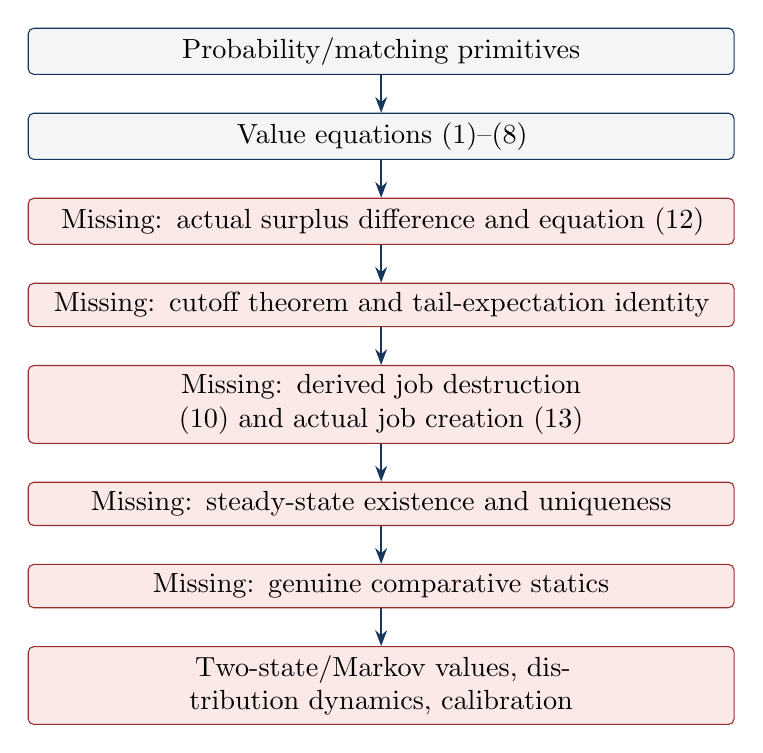
\begin{tikzpicture}[
  node distance=0.48cm,
  box/.style={draw=navy,rounded corners=2pt,fill=graybg,align=center,
              text width=0.72\linewidth,minimum height=0.55cm},
  miss/.style={draw=red,rounded corners=2pt,fill=redbg,align=center,
               text width=0.72\linewidth,minimum height=0.55cm},
  arr/.style={-{Stealth[length=2mm]},thick,navy}
]
\node[box] (p) {Probability/matching primitives};
\node[box,below=of p] (v) {Value equations (1)--(8)};
\node[miss,below=of v] (s) {Missing: actual surplus difference and equation (12)};
\node[miss,below=of s] (t) {Missing: cutoff theorem and tail-expectation identity};
\node[miss,below=of t] (j) {Missing: derived job destruction (10) and actual job creation (13)};
\node[miss,below=of j] (e) {Missing: steady-state existence and uniqueness};
\node[miss,below=of e] (c) {Missing: genuine comparative statics};
\node[miss,below=of c] (m) {Two-state/Markov values, distribution dynamics, calibration};
\draw[arr] (p) -- (v);
\draw[arr] (v) -- (s);
\draw[arr] (s) -- (t);
\draw[arr] (t) -- (j);
\draw[arr] (j) -- (e);
\draw[arr] (e) -- (c);
\draw[arr] (c) -- (m);
\end{tikzpicture}
\end{center}

\textbf{Three most important missing bridges}
\begin{enumerate}
  \item Actual \code{ValueEquilibrium.S} $\longrightarrow$ equation (12) and
  \code{S_cutoff}.
  \item Positive-continuation expectation $\longrightarrow$ tail-CDF integral,
  enabling (9) and (10).
  \item Derived JD/JC/Beveridge system $\longrightarrow$ existence and uniqueness of a
  steady state.
\end{enumerate}

\newpage
\section{First-milestone comparison}

\begin{longtable}{@{}p{0.23\linewidth}p{0.19\linewidth}p{0.23\linewidth}p{0.25\linewidth}@{}}
\toprule
\textbf{Candidate} & \textbf{Difficulty / risk} & \textbf{Immediate gain} & \textbf{Verdict} \\
\midrule
Probability/CDF foundation & Moderate-foundational; low circularity & Fixes atoms and
enables measure/Appendix work & Essential second track, but no immediate headline theorem. \\
Strengthen derivation of (8) & Elementary-moderate; low risk & Cleans an already proved
edge & Not the best new milestone. \\
Actual equation (12) & Elementary; low risk & First missing headline theorem; unlocks
actual JC and cutoff work & \gradegreen\ \textbf{Best first milestone}. \\
Derive equation (10) & Foundational; high premature-assumption risk & Major JD bridge &
Too early: tail identity and actual (12) missing. \\
Value-to-steady bridge & Foundational; high circularity risk & Closes architecture &
End of first proof phase, not first step. \\
\bottomrule
\end{longtable}

\section{Recommended next proof milestone}

\colorbox{greenbg}{\parbox{0.93\linewidth}{
\textbf{Prove the two-point surplus-difference form of equation (12) for the actual
\code{ValueEquilibrium.S}.}

For \code{A : Assumptions P} and \code{E : ValueEquilibrium P}, prove
\[
  E.S(\varepsilon_2)-E.S(\varepsilon_1)
  =\frac{\sigma(\varepsilon_2-\varepsilon_1)}{r+\lambda}.
\]
Use \code{E.surplus_bellman} at two shock values and subtract. Continuation and search
terms cancel, so no new measure theory is required.
}}

\textbf{Why it dominates.} It is upstream, elementary, noncircular, and establishes a
fact about the actual value equilibrium rather than another parallel formula. It unlocks
the actual equation (13) bridge, surplus monotonicity, and the next cutoff theorem. The
probability/CDF foundation should follow before tail-integral or derivative work.

\subsection*{First three milestones}

\begin{enumerate}
  \item \textbf{Actual equation (12):} two-point surplus difference, then equality with
  \code{S_cutoff}. Difficulty: elementary. Circularity risk: low.
  \item \textbf{Actual equation (13):} combine milestone 1 with zero profit and Nash
  sharing. Difficulty: elementary-moderate. Circularity risk: low.
  \item \textbf{Paper probability/CDF foundation:} probability instance, atomlessness,
  moments, and derived CDF facts. Difficulty: moderate-foundational. Circularity risk: low.
\end{enumerate}

\end{document}
